\documentclass[light]{lutbeamer} % change between light and dark for the background
%\documentclass[t]{lutbeamer} % use "t" option for top alignment 
\usepackage{caption}
\usepackage{xcolor}
\captionsetup{labelfont={color=gr},textfont={color=gr}}
\DeclareCaptionLabelFormat{nocolon}{#1 #2}
\captionsetup{labelformat=nocolon}
\usepackage{pgfpages}
\setbeameroption{hide notes} % Only slides
% \setbeameroption{show only notes} % Only notes
% \setbeameroption{show notes on second screen=right} % Both


\setdepartment{Data Science and Analytics Thrust, Information Hub}
\institute[HKUSTGZ]{The Hong Kong University of Science and Technology (Guangzhou)}
\author{Mingze Gong}
\title[GNNs for carbon emissions prediction]{AI-driven blockchain-based approach for car- bon market mechanism}
\subtitle{Graph Neural Networks for Spatial-Temporal Analysis and Prediction of Carbon Emissions in China’s Provinces}
\date{\today}


\begin{document}

% front page
{ % all template changes are local to this group.
\setbeamertemplate{navigation symbols}{}
\begin{frame}<article:0>[plain,noframenumbering]
    \begin{tikzpicture}[remember picture,overlay]
        \node[at=(current page.center)] {
            \includegraphics[
                width=\paperwidth,
                height=\paperheight]{figures/GZ Campus.jpeg}
        };
    \end{tikzpicture}
\end{frame}
}

% Outline
\AtBeginSection[]
{
    \begin{frame}[plain,noframenumbering]
        \frametitle{Outline}
        \begin{columns}[T]
            \begin{column}{0.01\textwidth}

            \end{column}
            \begin{column}{0.95\textwidth}
                \tableofcontents[currentsection,
                    %currentsubsection,
                    %hideothersubsections, 
                    %sectionstyle=show/sh ed, 
                    %subsectionstyle=show/shaded%/hide
                ]
            \end{column}
        \end{columns}
    \end{frame}
}

{ % title page
    \begin{frame}[plain]
        \maketitle
        \small
        \par\vskip-0.1em
        {\footnotesize
        \begin{beamercolorbox}[sep=8pt,left]{author}
            \usebeamerfont{author}{Presented by \insertauthor} on \insertdate
        \end{beamercolorbox}%\vskip0.5em
        }
        \note{
            Dear Professors, Dr. Li and Dr. Zhang, Good morning, given the group project, I will be presenting my individual topic. \\~\\

            I will start with the project overview.
        }

    \end{frame}
}
% % % % % % % % % % % % % % % % % % % % % % % % % % % % % % % % % % % %
\section{Introduction}
\subsection{Group Project Overview}
\begin{frame}
    \frametitle{Project Overview}
    \framesubtitle{Bridging Individual and Group Efforts}
    \begin{columns}
        \begin{column}{0.4\textwidth}
            \begin{itemize}
                \item My role: \alert{Spatial-temporal analysis} and \alert{prediction} of carbon emissions.
                \item Targets: \alert{Accurate and efficient} emission predictions to inform the market mechanism.
                \item Contributions: Enhance \alert{decision-making} and optimize carbon \alert{trading strategies}.
                \item Relationship: Provide \alert{data-driven insights} for the group project
            \end{itemize}
        \end{column}
        \begin{column}{0.6\textwidth}
            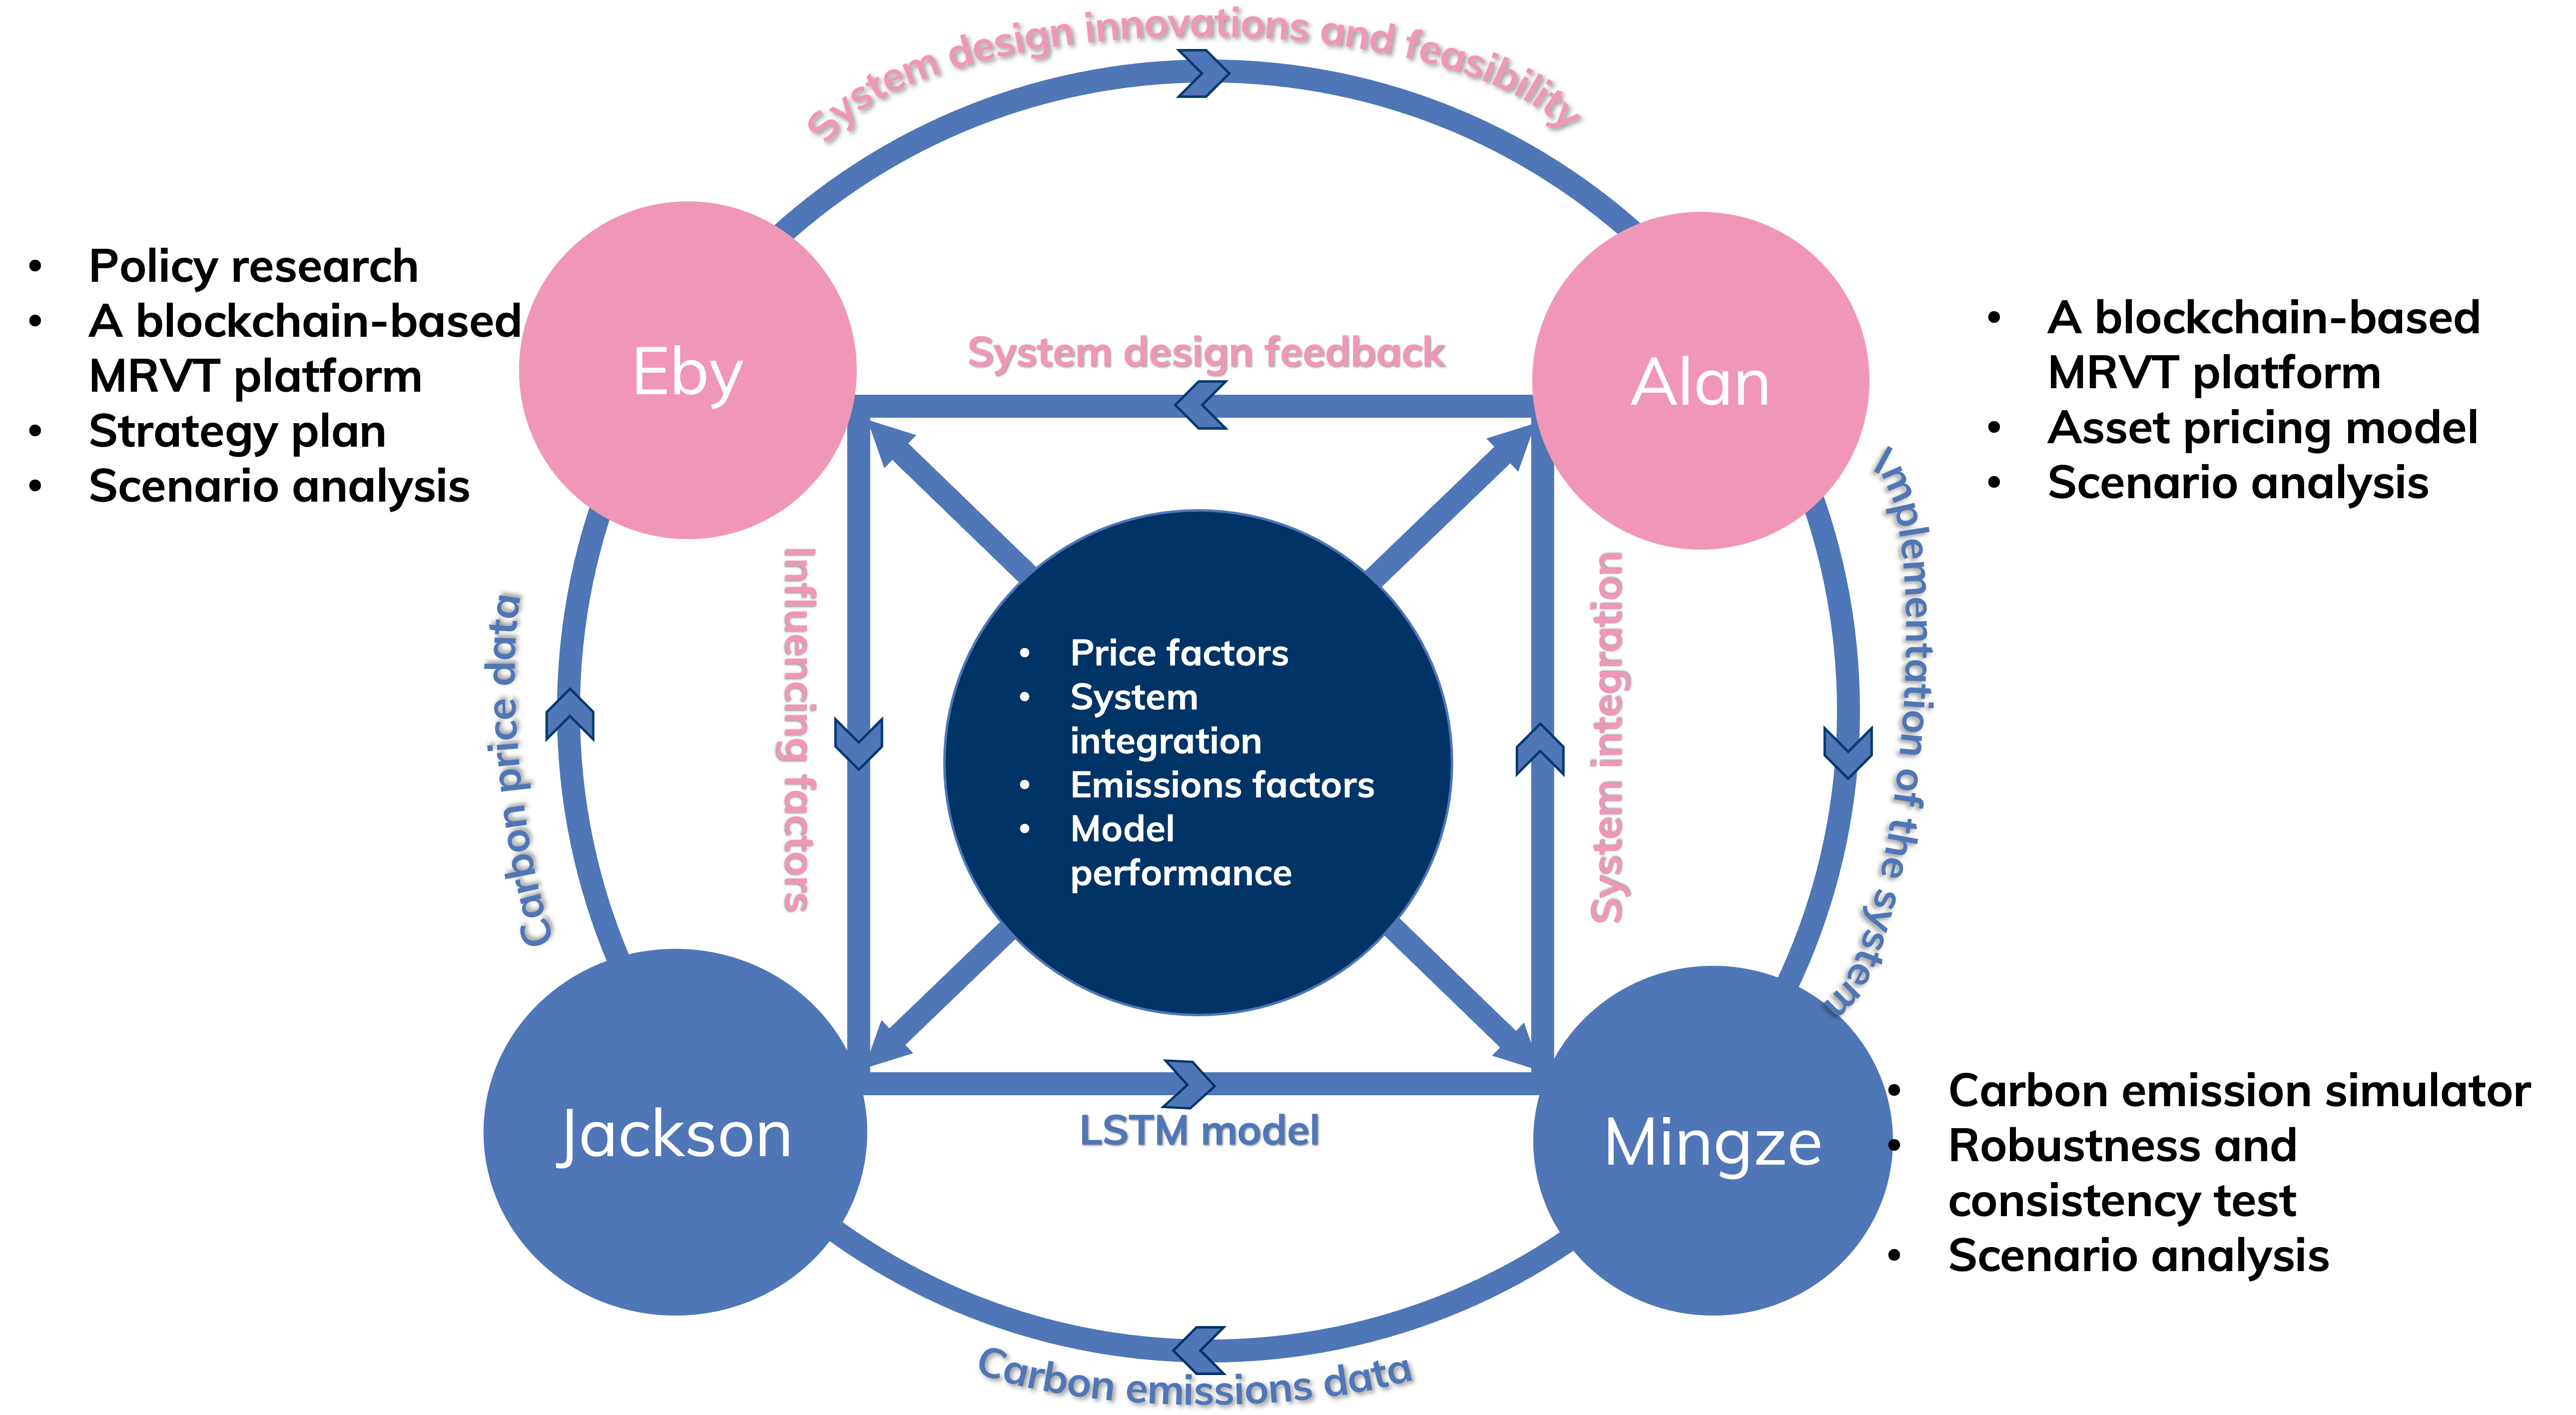
\includegraphics
            [width=\textwidth]{figures/team_collaboration.png}
            \captionof{figure}{Team Collaboration Chart}
        \end{column}
    \end{columns}
    \note{
        As part of this project, I have taken on the responsibility of conducting spatial-temporal analysis and prediction of carbon emissions, particularly by using GNN. \\~\\

        The primary target of my project is to achieve accurate emission prediction which will serve as the foundation for the carbon market mechanism, ensuring fair and transparent carbon pricing. \\~\\

        My contribution is centered around enhancing decision-making and optimizing carbon pricing and trading strategies.  \\~\\

        The relationship lies in the data-driven insights I provide. It will ensure the mechanism is based on reliable and up-to-date information.\\~\\
    }
\end{frame}
% % % % % % % % % % % % % % % % % % % % % % % % % % % % % % % % % % % %
\subsection{Introduction to Individual Project}

\begin{frame}
    \frametitle{Introduction to Individual Project}
    \framesubtitle{Carbon Emissions Prediction}

    \begin{minipage}[t][0.6\textheight]{0.45\textwidth}
        \textbf{Background}
        \begin{itemize}
            \item Disrupted balance between "growth and consumption"
            \item The necessity of limiting global warming to
                  1.5°C above pre-industrial levels
            \item China's determination to achieve sustainable development
        \end{itemize}
    \end{minipage}
    \hfill
    \begin{minipage}[t][0.6\textheight]{0.45\textwidth}
        \textbf{Significance}
        \begin{itemize}
            \item Valuable insights for various stakeholders
            \item Climate change modelling
            \item Governments' and public's awareness
        \end{itemize}
    \end{minipage}
    \note{
        Now let's dive into my individual project.  \\~\\
        
        I wanna briefly talk about the research background and significance. \\~\\

        The balance between "growth and consumption" has been disrupted, and the world is facing the necessity of limiting global warming. In addition, China has accelerated the implementation of its "dual carbon" goal.\\~\\

        Why is this research important then? \\~\\

        First of all, emission prediction is valuable for various stakeholders, including governments, industries, and researchers, providing insights for them and allowing them to make informed decisions.\\~\\

        It's also crucial for climate change modeling as it helps to estimate future greenhouse gas concentrations in the atmosphere. \\~\\

        Lastly, it can raise public awareness about the urgency of climate change and the need for immediate action. Sustainable practices will be encouraged. \\~\\
    }

\end{frame}

% % % % % % % % % % % % % % % % % % % % % % % % % % % % % % % % % % % %
\section{Literature Review}
\subsection{Prior research on carbon emissions}
\begin{frame}
    \frametitle{Literature Review}
    \framesubtitle{Various purposes}
    \begin{itemize}
        \item China’s transportation carbon emissions and influencing factors \cite{cai2022-spatialtemporal}
        \item The relationship between land use and carbon emissions \cite{huang2022-study}
        \item Spatial pattern of carbon emissions in Nanjing \cite{wu2022-prediction}
        \item The relationship between economic development and carbon emissions \cite{yin2022-spatial}
        \item ...
    \end{itemize}
    \note{
        Prior research on carbon emissions showcases varuous purposes. \\~\\

        Some had tried to analyze the transportation carbon emissions and its influencing factors, while others studied the relationship between land use and carbon emissions, the spatial pattern of carbon emissions etc.
        \\~\\
    }
\end{frame}

\begin{frame}
    \frametitle{Literature Review}
    \framesubtitle{Plenty of Models}
    \begin{minipage}[t][1\textheight]{0.47\textwidth}
        \textbf{Statistical Methods}
        \begin{itemize}
            \item \emph{STIRPAT model} for emissions in Qingdao \cite{wu2018-scenario}
            \item \emph{Grey forecasting model} for small sample data \cite{ju-long1982-control}
            \item A \emph{dynamic time-delay discrete grey forecasting model} for time-lag effects \cite{ye2022-enhanced}
            \item \emph{ARIMA model} for emissions in four representative provinces and cities \cite{ning2021-forecast}
            \item \emph{A novel fractional grey Riccati model} for emission prediction in US, China and Japan\cite{gao2021-novel}
        \end{itemize}
    \end{minipage}
    \hfill
    \begin{minipage}[t][1\textheight]{0.47\textwidth}
        \textbf{Machine Learning Methods}
        \begin{itemize}
            \item \emph{SVM-ELM model} to forecast emissions in specific regions \cite{li2018-forecasting}
            \item A \emph{BP neural network model} for emissions in Beijing \cite{liu2018-regional}
            \item \emph{PCA and regularized extreme learning machine} in a hybrid prediction model for China's emission \cite{sun2017-prediction}
            \item \emph{ENN model} for emissions in China \cite{zhou2019-forecasting}
            \item \emph{A hybrid Fast Learning Network–Chicken Swarm Optimization model} for emissions in Guangdong \cite{ren2021-carbon}
        \end{itemize}
    \end{minipage}
    \note{
        Regarding prediction, there's basically two categories of models, statistical and machine learning models. \\~\\
        Grey forecasting model and ARIMA are very popular. \\~\\
        About machine learning models, BP neural network, ENN, and hybrid model are investigated a lot. \\~\\
    }
\end{frame}

\begin{frame}
    \frametitle{Literature Review}
    \framesubtitle{Graph Neural Networks (GNNs)}

    \begin{minipage}[c]{0.65\textwidth}
        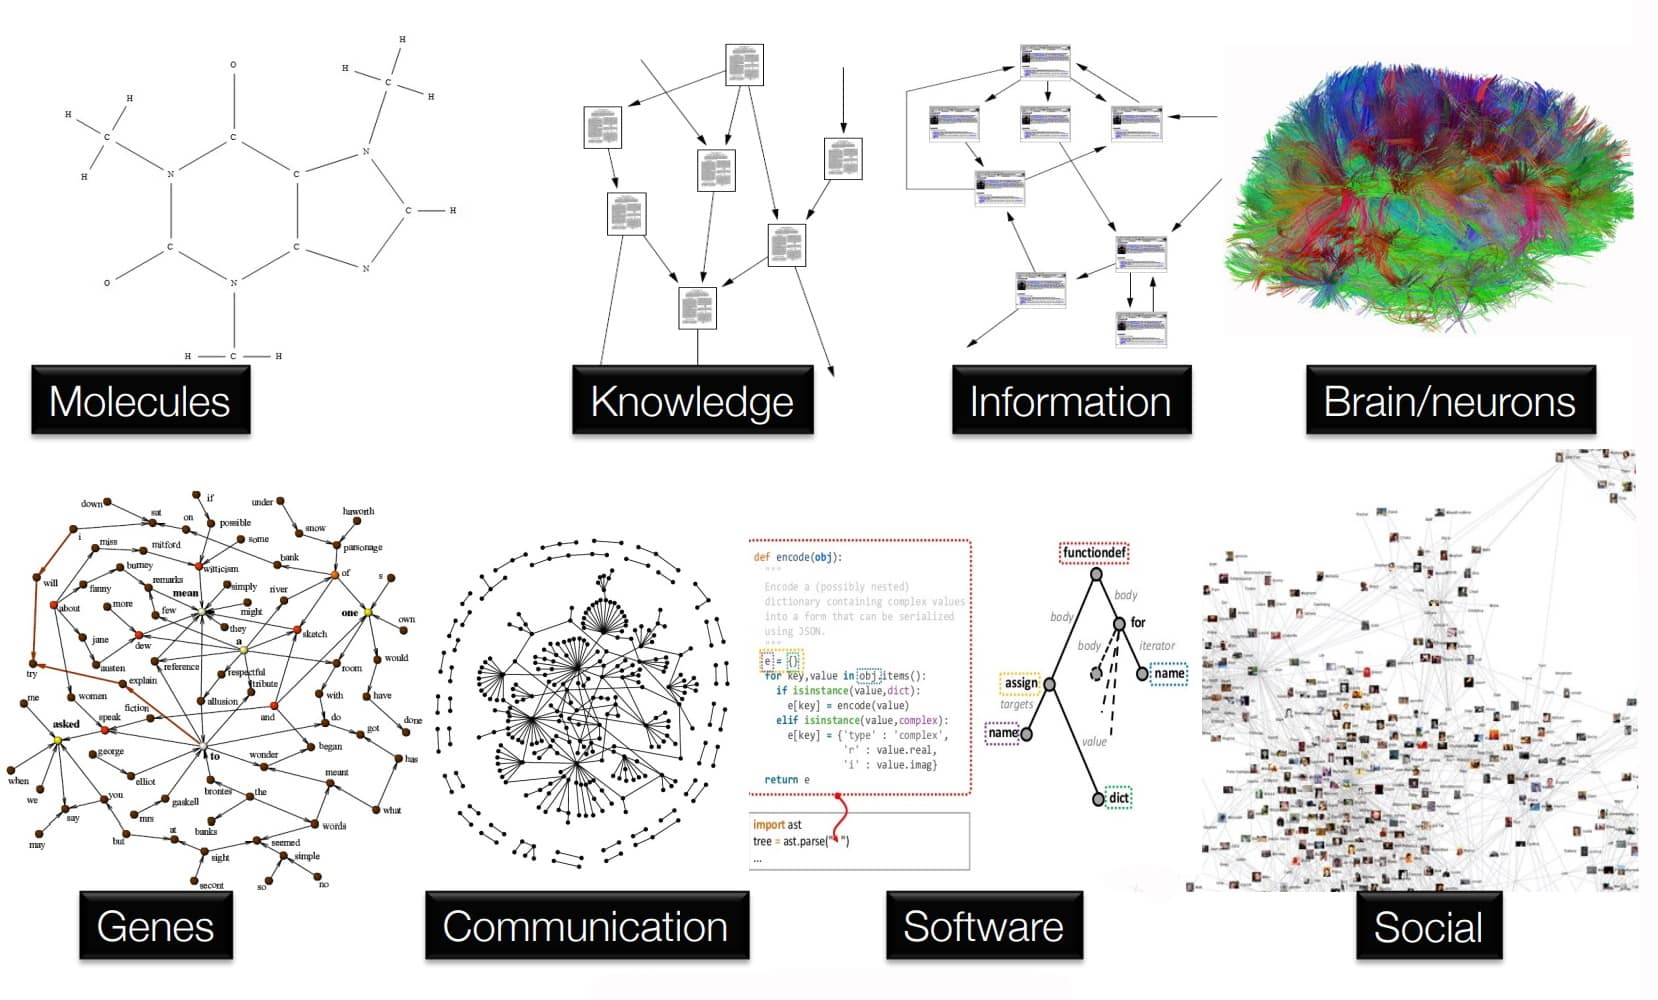
\includegraphics[width=\textwidth]{figures/what_is_GNNs.jpeg}
        \vspace{-0.5cm} % Adjust vertical space
        \captionof{figure}{Knowledge from many fields of science and industry can be expressed as graphs \cite{merritt2022-what}}
    \end{minipage}
    \hfill
    \begin{minipage}[c]{0.3\textwidth}
        Two types of application scenarios \cite{zhou2020-graph}
        \begin{itemize}
            \item Structural data
                  \begin{itemize}
                      \item Graph matching, clustering etc.
                      \item Traffic, knowledge graph etc.
                  \end{itemize}
            \item Non-structural data
                  \begin{itemize}
                      \item Image
                      \item Text
                  \end{itemize}
        \end{itemize}
    \end{minipage}
    \note{
        Generally speaking, Ml models outperforms statistical modles due to their ability to capture non-linear relationships between carbon emissions and weather like temperature or else. \\~\\
        Among all of them, Graph Neural Networks, a data structure consisting of nodes and edges, have become increasingly popular thanks to its expressive power across various fields. Social science, natural science, knowledge graphs, and other research areas have utilized graphs to represent their own systems. \\~\\
        Its applications can be grouped into two categories: structural and non-structural. Structural data is represented by something that could be converted to graphs like traffic and social network, while non-structural data is represented by images or text, which I believe are two of the most active branches of AI research at this moment. \\~\\
        There's quite a lot of research on application of GNNs in various scenarios and there is no doubt that it can better capture the spatial and temporal dependencies. But very few research was found in carbon emission forecasting. I beileve this is related to the limited dataset and difficulty of constructing a meaningful graph structure. \\~\\
        
        These are something we're going to focus on in the next couple of months. \\~\\
    }

\end{frame}

% % % % % % % % % % % % % % % % % % % % % % % % % % % % % % % % % % % % 
\section{Research Objectives and Questions}
\subsection{Main Objectives}
\begin{frame}
    \frametitle{Research Objectives and Questions}
    \framesubtitle{Main Objectives}
    \begin{enumerate}
        \item To construct a comprehensive carbon emission dataset for training and testing the GNN model.
        \item To investigate the potential of GNNs in predicting carbon emissions.
        \item To identify the key factors and variables that influence carbon emissions and can be effectively incorporated into the GNN model.
        \item To develop a robust GNN model that accurately predicts carbon emissions and outperforms traditional forecasting statistical methods and other machine learning methods.
        \item To provide insights and recommendations for policy-makers and stakeholders based on the GNN model's predictions to facilitate effective carbon emission reduction strategies.
    \end{enumerate}
    \note{
        The main objectives of this research are to construct a comprehensive  emission dataset for training and testing the GNN model, to investigate the potential of GNN in emission prediction, to identify the key factors that influence emissions, to develop a robust GNN model that outperforms traditional statistical and other ML methods, and to provide insights for stakeholders around emission reduction strategies. \\~\\
    }
\end{frame}

\subsection{Research Questions}
\begin{frame}
    \frametitle{Research Objectives and Questions}
    \framesubtitle{Research Questions}
    \begin{enumerate}
        \item What are the most influential variables and features that should be incorporated into the GNN model to enhance its prediction accuracy?
        \item How can GNNs be applied to predict carbon emissions effectively, considering the non-linearity characteristics of carbon emission data and related features?
        \item How does the performance of the GNN model compare with traditional forecasting methods in predicting carbon emissions, and what are the advantages and limitations of using GNNs in this context?
        \item How can the predictions generated by the GNN model be used to inform policy-makers and stakeholders in designing and implementing effective carbon emission reduction strategies?
        \item Are there any potential challenges or limitations in using GNNs for carbon emission prediction, and how can these be addressed to improve the model's performance and reliability?
    \end{enumerate}
    \note{
        Around previous objectives, the following questions are raised to guide the research. \\~\\
        
        What are the most influential variables? How can GNNs be applied, considering the non-linearity characteristics? Compared with traditional methods, how does it perform? How can stakeholders be informed? Any potential limitations there? \\~\\
    }
\end{frame}
% % % % % % % % % % % % % % % % % % % % % % % % % % % % % % % % % % % %
\section{Preliminary Findings}
\subsection{Accomplished work}
\begin{frame}
    \frametitle{Summary Of Accomplished Work}
    \framesubtitle{A Comprehensive Literature Review}
    \centering
    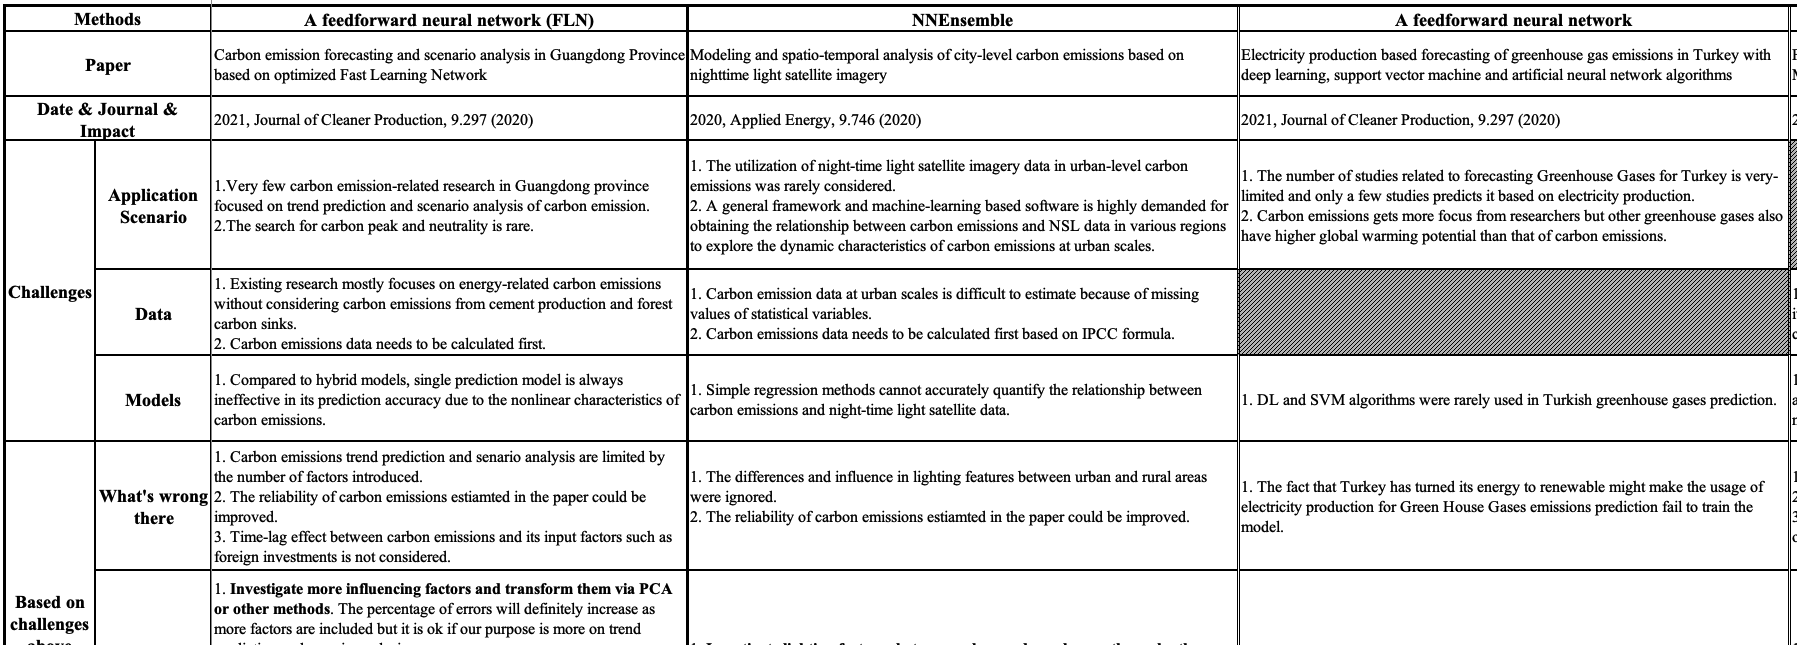
\includegraphics[width=\textwidth]{figures/summary_previous_work.png}
    \vspace{-0.2cm} % Adjust vertical space
    \captionof{table}{A partial screenshot of the summary based on comprehensive literature review regarding emission prediction}

    \note{
        The following section talks about some preliminary findings since this February. \\~\\

        With my supervisors' and Dr. Zhang's help, I've conducted a comprehensive review around emission prediction. Application scenarios, data sources, specific models employed, present challenges etc. All was summarised and could be referred to in my written proposal Appendix A and this is just a screenshot. \\~\\
    }
\end{frame}

\subsection{Initial Thoughts}
\begin{frame}
    \frametitle{Summary Of Accomplished Work}
    \framesubtitle{Initial Thoughts}
    \begin{minipage}[c]{0.45\textwidth}
        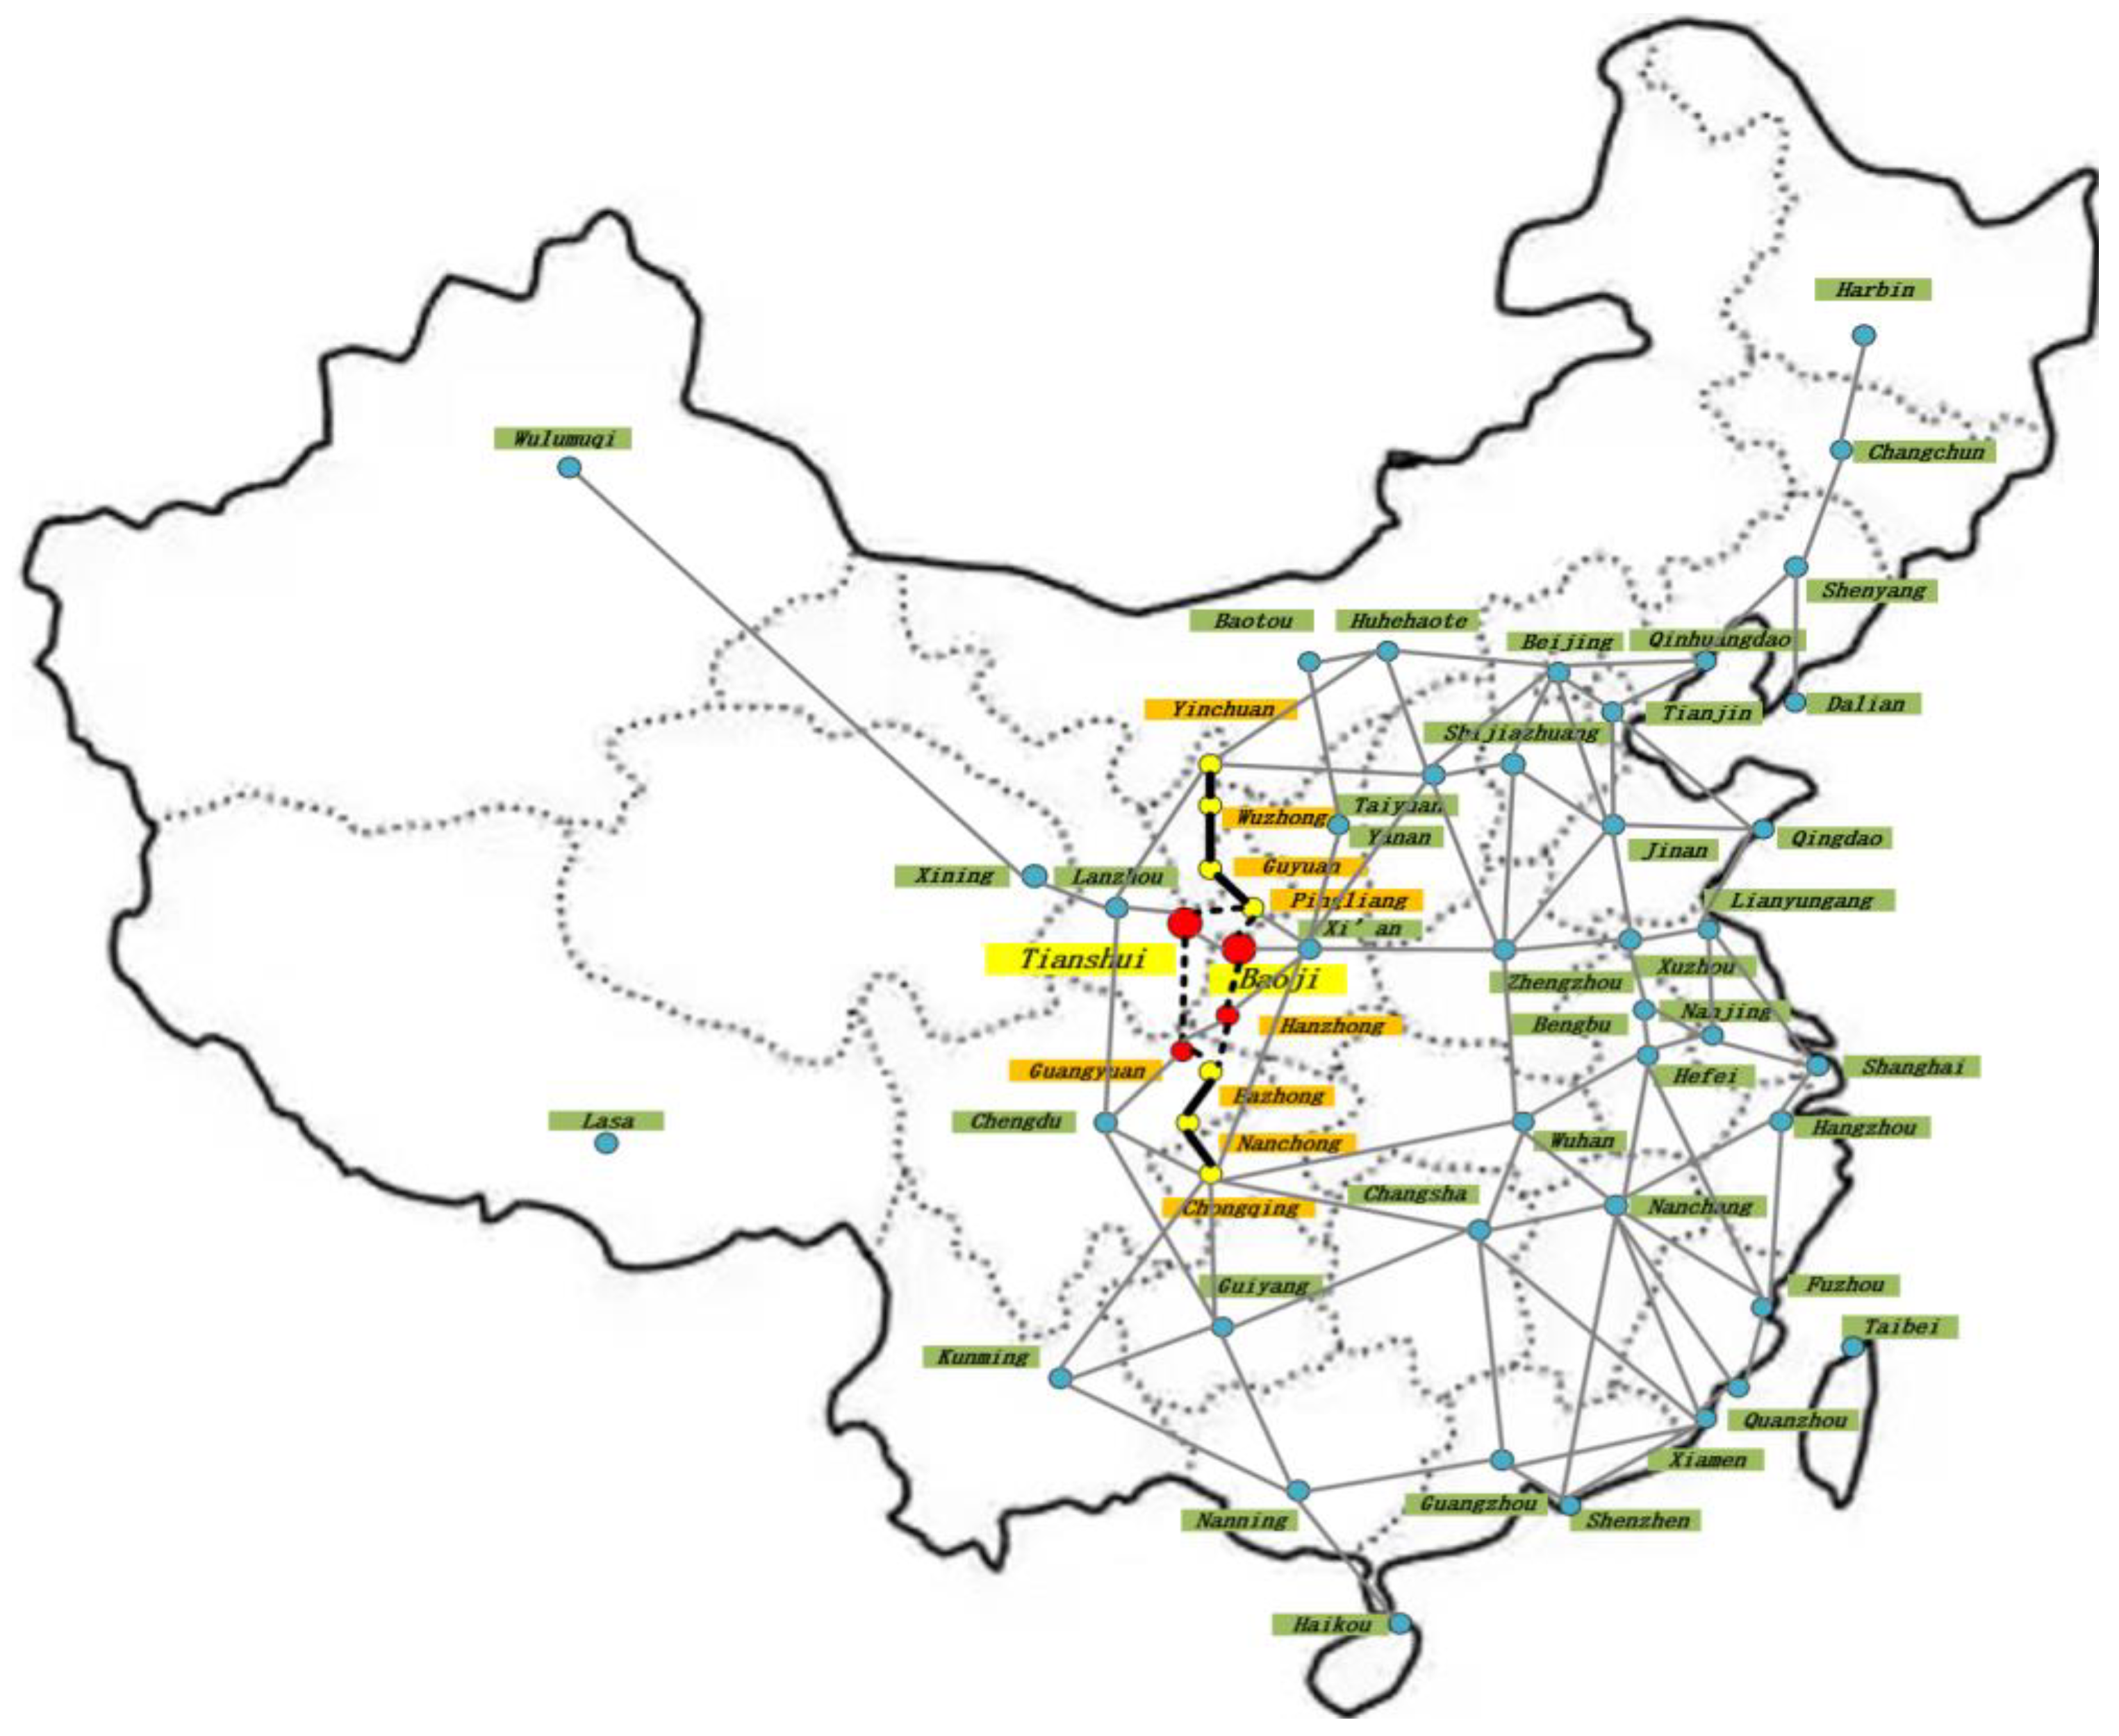
\includegraphics[width=\textwidth]{figures/province_edge.png}
        \captionof{figure}{A figure showing the connection between each province in China \cite{ma2023-scattergnn}}
    \end{minipage}
    \hfill
    \begin{minipage}[c]{0.45\textwidth}
        Two approaches for similarities measurement
        \begin{itemize}
            \item \alert{Features/Factors-based Approach}
                  \begin{itemize}
                      \item Node features
                      \item Edge features
                  \end{itemize}
            \item Index-based Approach
                  \begin{itemize}
                      \item Euclidean distance
                      \item Jaccard index
                  \end{itemize}
        \end{itemize}
    \end{minipage}

    \note{
        After the review, I think the key to employing GNNs for emission prediction is to construct a graph where edges connect provinces based on their similarities which could be measured using two approaches: Features-based and Index-based. \\~\\

        For the feature-based approach, we can gather several influencing features, such as GDP, population etc. They can then be categorized into node features and edge features. Once features are confirmed and the weights are assigned, the similarities between provinces could be determined. \\~\\

        An alternative approach is using Euclidean distance or Jaccard index to measure. But, I think it's a bit redundant in some way. And I may focus more on the first approach later. \\~\\
    }
\end{frame}

\subsection{Code Testing}
\begin{frame}
    \frametitle{Summary Of Accomplished Work}
    \framesubtitle{Hands-on Experience}
    \begin{minipage}[c]{0.45\textwidth}
        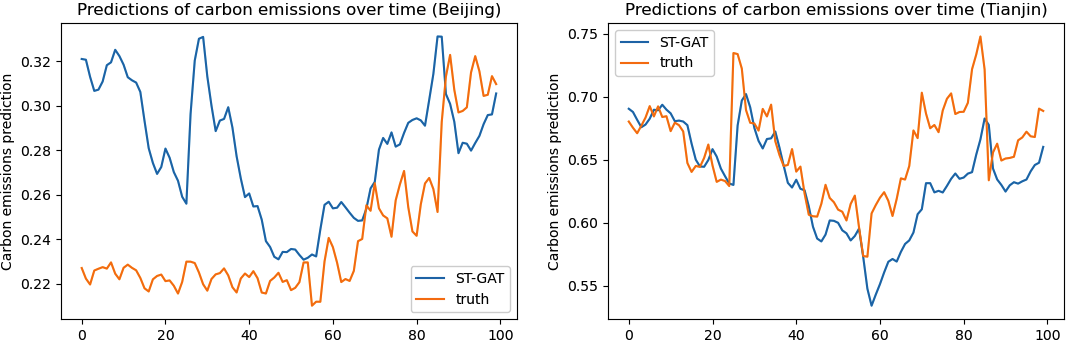
\includegraphics[width=\textwidth]{figures/prediction_baseline.png}
        \captionof{figure}{STGAT Baseline Model : Partial Performance (Beijing and Tianjin) in Predicting Carbon Emissions.}
        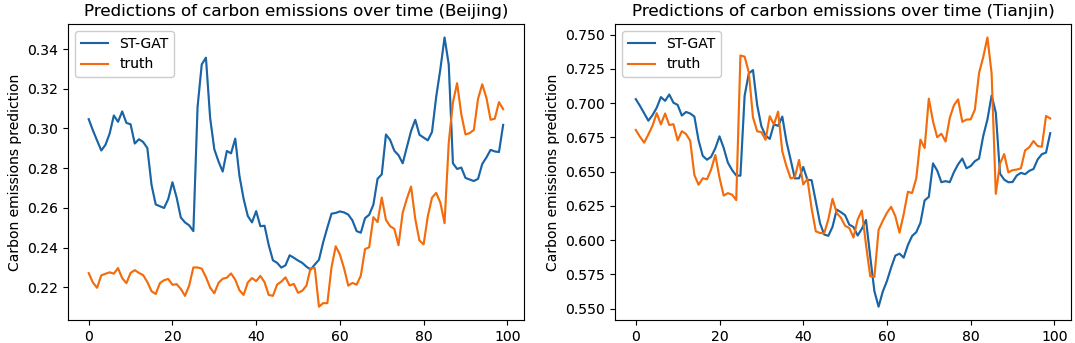
\includegraphics[width=\textwidth]{figures/prediction_grp.png}
        \captionof{figure}{STGAT Model with GDP Feature: Partial Performance (Beijing and Tianjin) in Predicting Carbon Emissions.}
    \end{minipage}
    \hfill
    \begin{minipage}[c]{0.5\textwidth}
        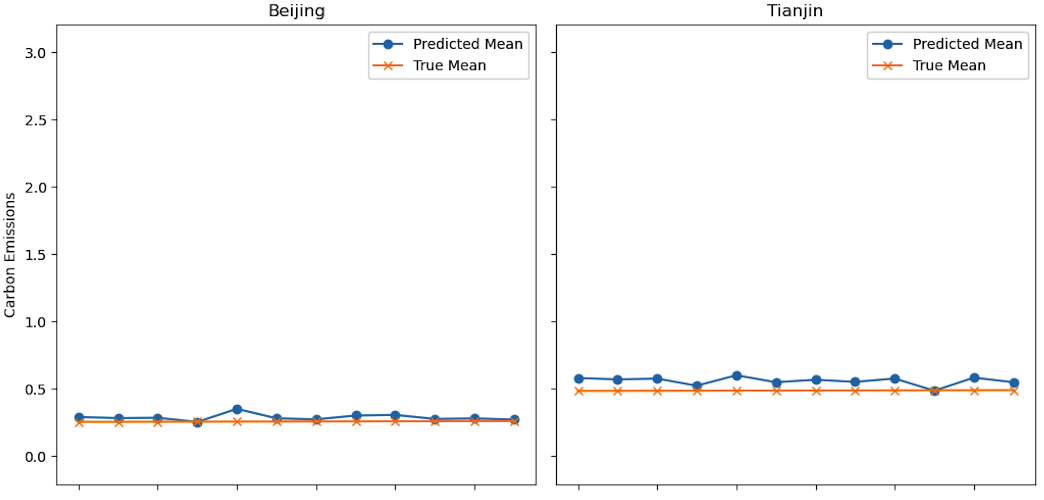
\includegraphics[width=\textwidth]{figures/AGCRN.png}
        \captionof{figure}{AGCRN Model: Partial Performance (Beijing and Tianjin) in Predicting Carbon Emissions.}
    \end{minipage}
    \note{
        I have also tried to implement some GNN models. But because there are almost no literature on emission prediction by GNN, I have to first try traffic datasets instead. After testing successfully, I tried the carbon datasets. \\~\\

        I've successfully tested two models basically, one with Spatial Temporal Graph Attention model and the other with Adaptive Graph Convolutional Recurrent Network. The organge line is ground truth while the blue one is predicted values. They have different forecast horizon. Considering the time, I didn't adjust them to be the same. And these are only the results of 2 out of 31 provinces\\~\\

        Overall, the performance is quite bad honestly but this has been anticipated since we haven't tuned the model and just wanna have a look how it goes when using GNNs on carbon emissions. It seems that there's still big improvements to be made. \\~\\
    }
\end{frame}
% % % % % % % % % % % % % % % % % % % % % % % % % % % % % % % % % % % %
\section{Research Plan}
\begin{frame}
    \frametitle{Research Plan}
    \framesubtitle{}
    \begin{minipage}[c]{0.45\textwidth}
        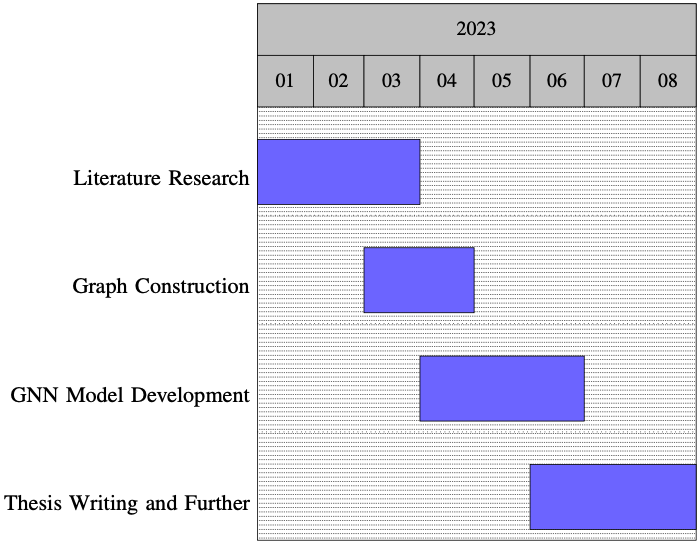
\includegraphics[width=\textwidth]{figures/Gannt.png}
        \captionof{figure}{\raggedleft Gantt chart for my research plan.}
    \end{minipage}
    \hfill
    \begin{minipage}[c]{0.45\textwidth}
        \begin{itemize}
            \item \alert{2023.01-2023.03}
                  \begin{itemize}
                      \item Literature Research
                      \item Data Preprocessing
                  \end{itemize}
            \item \alert{2023.03-2023.04}
                  \begin{itemize}
                      \item Codes Testing and Feature Selection
                      \item Graph Construction
                  \end{itemize}
            \item \alert{2023.04-2023.06}
                  \begin{itemize}
                      \item GNN Model Development, Training, Evaluation
                      \item Models Comparison
                  \end{itemize}
            \item \alert{2023.06-2023.08}
                  \begin{itemize}
                      \item Thesis Writing and Further
                  \end{itemize}
        \end{itemize}
    \end{minipage}

    \note{
        Next is my draft research plan. I am now testing some codes and doing the feature selection with more meaningful graphs to be made. Hopefully, some concrete results could be presented by the end of June and I'll start writing my thesis. \\~\\
    }

\end{frame}
% % % % % % % % % % % % % % % % % % % % % % % % % % % % % % % % % % % %
\section{Potential challenges and solutions}
\subsection{Anticipated Issues Potential Solutions}
\begin{frame}
    \frametitle{Potential challenges and solutions}
    \framesubtitle{Anticipated Issues and Potential Solutions}
    \begin{minipage}[t]{0.45\textwidth}
        \textbf{Anticipated Issues}
        \begin{itemize}
            \item Limited existing research on GNNs for carbon emissions prediction.
            \item Scarce high-dimensional GNN models built upon multiple edge features.
            \item Data quality and availability.
            \item Computational complexity.
        \end{itemize}
    \end{minipage}
    \hfill
    \begin{minipage}[t]{0.45\textwidth}
        \textbf{Potential Solutions}
        \begin{itemize}
            \item An extensive literature review on related fields where GNNs have been applied.
            \item Thorough data preprocessing and cleaning to ensure the consistency and accuracy.
            \item GNN model optimization for computational complexity reduction.
        \end{itemize}
    \end{minipage}

    \note{
        Lastly, I wanna end this presentation with some identified challenges. First and foremost, there are very limited existing research and datasets on carbon emissions prediction by GNN. I think this is the most challenging part. Although some methods might be applicable, like the ones on traffic prediction, it is uncertain whether these methods can be directly translated into carbon emissions prediction.\\~\\
        Then, the incorporation of multiple edge features demands the development of a higher-dimensional GNN model, which may pose challenges in model design and optimization. \\~\\
        Obtaining high-quality and consistent data for all 31 provinces might pose a challenge as well. \\~\\
        Finally, the high-dimensional GNN model could necessitate sinificant computational resources, potentially affecting the model’s scalability. \\~\\
        Accordingly, my proposed solutions include a more extensive review and thorough data preprocessing. And I am now learning to trade modles via cloud platform to improve the efficiency. \\~\\
    }
\end{frame}

% % % % % % % % % % % % % % % % % % % % % % % % % % % % % % % % % % % %


\appendix % to start a separate page numbering

\section*{Bibliography}
\begin{frame}[allowframebreaks]
    \textbf{References}
    \printbibliography
\end{frame}


{ % all template changes are local to this group.
\setbeamertemplate{navigation symbols}{}
\begin{frame}<article:0>[plain,noframenumbering]
    \begin{tikzpicture}[remember picture,overlay]
        \node[at=(current page.center)] {
            
\includegraphics[
                width=\paperwidth,
                height=\paperheight]{figures/ThankYouPage.png}
        };
    \end{tikzpicture}
    % \begin{tikzpicture}[remember picture,overlay]
    %     \node[at=(current page.center)] {
    %         
\includegraphics[keepaspectratio,
    %             width=0.65\paperwidth,
    %             height=\paperheight]{figures/ThankYouPage.png}
    %     };
    % \end{tikzpicture}
\end{frame}
}

\end{document}
